\documentclass[12pt]{article}

\usepackage[utf8]{inputenc}
\usepackage{amsmath,amsfonts,amssymb,amstext}
\usepackage{fullpage}
\usepackage{hyperref}

% make things look prettier
\usepackage{tabulary,colortbl}
\usepackage{textcase}
\usepackage{multirow}
\usepackage{booktabs}
\usepackage{centernot}
%\usepackage{microtype}
\usepackage{nicefrac}
\usepackage[table]{xcolor}
\definecolor{darkblue}{rgb}{0,0,0.5}
\definecolor{darkgreen}{rgb}{0,0.5,0}
\usepackage{xspace}
\usepackage{url}
\usepackage{esvect}
\usepackage{tikz}
\usepackage{algorithm}
\usepackage[noend]{algorithmic}


\xdefinecolor{redx}{rgb}{1,0,0}
\xdefinecolor{greenx}{rgb}{0,.7,0}
\xdefinecolor{bluex}{rgb}{0,0,.8}
\xdefinecolor{purplex}{rgb}{.7,0,.7}
\xdefinecolor{orangex}{rgb}{.9,.5,0}

\newcommand{\rgrey}[1]{{\color{greyx!40}#1}}
\xdefinecolor{greyx}{rgb}{0,0,0}

\newcommand{\rred}[1]{{\color{redx!100}#1}}
\newcommand{\ggreen}[1]{{\color{greenx!100}#1}}
\newcommand{\bblue}[1]{{\color{bluex!100}#1}}
\newcommand{\ppurple}[1]{{\color{purplex!100}#1}}
\newcommand{\oorange}[1]{{\color{orangex!100}#1}}


\renewcommand{\vec}{\mathbf}
\renewcommand{\algorithmicrequire}{\textbf{Input:}}
\renewcommand{\algorithmicensure}{\textbf{Output:}}
\newcommand{\ps}[2]{\langle {#1}, {#2} \rangle}

\newcommand{\Z}{\mathbb Z}
\newcommand{\R}{\mathbb R}
\newcommand{\Ball}{\mathfrak B}
\newcommand{\norm}[1]{\|#1\|}
\newcommand{\Span}{\ensuremath{\operatorname{Span}}}
\global\long\def\cL{\mathcal{L}}
\global\long\def\cP{\mathcal{P}}
\global\long\def\cF{\mathcal{F}}
\global\long\def\Id{\vec I}


\newtheorem{theorem}{Theorem}{\bfseries}{\upshape}
\newtheorem{lemma}[theorem]{Lemma}{\bfseries}{\upshape}
\newtheorem{prob}{Problem}{\bfseries}{\upshape}
\newtheorem{definition}{Definition}{\bfseries}{\upshape}
\newtheorem{claim}[theorem]{Claim}{\bfseries}{\upshape}
\newtheorem{fact}[theorem]{Fact}{\bfseries}{\upshape}
\newtheorem{proposition}[theorem]{Proposition}{\bfseries}{\upshape}
\newtheorem{problem}{Problem}{\bfseries}{\upshape}
\newtheorem{corollary}[theorem]{Corollary}{\bfseries}{\upshape}
\newtheorem{heuristic}{Heuristic}{\bfseries}{\upshape}
\newtheorem{oprob}{Open Problem}{\bfseries}{\upshape}
\newenvironment{proof}{\paragraph{Proof:} }{\hfill\qed\\}
\newcommand{\qed}{\hfill \ensuremath{\Box}}
\newcommand{\Vol}{\operatorname{Vol}}


\newcommand{\half}{\ensuremath{\nicefrac 1 2}}
\newcommand{\nicehalf}{\ensuremath{\nicefrac 1 2}}
\newcommand{\halfinterval}{\ensuremath{[\mbox{-} \half,\half)}}


\title{A brief introduction to lattices  for cryptography}
\author{L\'eo Ducas}
\date{Lecture notes from The African Mathematical School \\ Bamenda, Cameroon, June 2016}
\begin{document}
\maketitle

\section{Introduction}

\paragraph{Cryptography}

Cryptography is the art of keeping communication confidential and secure. Those properties are provided by the two basic primitives: encryption and signatures. Here we are only interested in {\em asymmetric cryptography}: there should be two keys, a private or secret one, allowing its owner the decrypt or to sign, while the public key, which is given to everyone allows only to encrypt or to verify signatures.

Cryptography is used behind the scene each time we use our credit-card or connect to a website using the protocol \texttt{https}. Without secure cryptography, many infrastructure, including internet, would completly fall apart, making them vulnerable to attacks from hackers, totalitarian government, or rogue agencies.

To ensure that those schemes are unbreakable, cryptography relies on mathematical problems that are hard to solve. By hard, it should be understood that, given a computer, solving those problems would take millions or billions of years. More formally, cryptosystems are defined with a security parameter $\kappa > 0$, and it should be the case that the problems take exponential time $2^\kappa$ to solve given only the public key, but can be solve in polynomial time $\kappa^c$ for some small constant $c$ given the secret key.

To build such cryptosystems, one must find a mathematical structure that can be described simply, but for which some special information (the secret key) allows to do some computation that is otherwise intractable. The simplest and oldest example of such structure is an RSA modulus: the ring $\Z / N\Z$ for a composite integer $N = pq$ where $p$ and $q$ are primes. In that case the special knowledge is the factorization $p$ and $q$. While $N$ easily allows to encrypt a message $\mathcal E_N : m \rightarrow m^e \bmod N$, the knowledge of $p$ and $q$ allows to inverse the above function, by computing an inverse exponent $d$ such that $ed = 1 \bmod (p-1)(q-1)$.

\paragraph{Motivations}

The RSA cryptosystem is nowadays considered quite inefficient: public-keys are large, and computations are slow. The best cryptosystems currently in use are based on elliptic curves.

Alternatives to RSA and elliptic curves have been studied, based on codes, or on lattices for example. There are many motivation to develop new cryptosystems, such as improving efficiency, or adding new functionalities. Lattice-based-cryptography has been very successful in that regard: for example the NTRU-Encrypt scheme, based on lattices with special structures is one of the fastest scheme for that task. Another breakthrough in cryptography that came from lattices is the realization of fully-homomorphic encryption (FHE). In such an encryption scheme, one can compute ``through'' the encryption, that is can compute any function on ciphertexts without learning the content of the ciphertexts. This allows a lot of flexibility when using cryptography, for example when one party one to delegate computation to someone else, while keeping its data private.

Another advantage of lattice-based cryptography is that it also seems to be resistant to quantum algorithms. While the quantum computer is not working today, such computer would be able to easily break RSA and elliptic curve based cryptosystems. If it is to be realized in the next decades, we must prepare for it as soon as possible. This is another reason Lattice-based cryptography has grown very popular over the last few years.

\paragraph{This lecture.}

In most of the literature on lattice-based cryptography, an algebraic presentation is chosen, and often lattices are not even defined, and it is not always obvious to understand how those cryptosystems are connected with lattices. 

While this presentation is convenient to build more and more advanced cryptosystems, the general ideas and intuitions behind those construction are not so explicit. 

In this lecture we chose to instead really start from the geometric point on view on lattices, and see how those ideas naturally lead to construction of lattice-based cryptosystems. We therefore choose to be somehow formal on the definition of lattices and there properties, but will just give an overview of lattice based cryptography.

The intent is to give an intuitive geometric guide to understand recent research articles on lattice based cryptography despite their algebraic presentation. Such articles typically speaks of the Short Integer Solution problem (SIS), the Learning with Error problem (LWE), their ring variants, and the NTRU cryptosystem. 

\paragraph{Additional resources}

The sources of this lecture notes, and other documents associated with those lectures are available online~\footnote{\url{https://github.com/lducas/bamenda}}, including the slides on cryptography, and the solution in \texttt{gp} to the programming exercises.

A significant portion of those notes are adapted from the Chapter 2 of my Ph.D. thesis\footnote{\url{http://homepages.cwi.nl/~ducas/Thesis/index.html}}, where one may find a more complete presentation of lattices and lattice-based cryptography. It was also inspired by the lecture notes of Daniele Micciancio\footnote{\url{http://cseweb.ucsd.edu/classes/sp14/cse206A-a/index.html}}. Both are available online (see the reference section). 

For a more advanced course on lattices (with less cryptography) on can also study the lectures notes of Oded Regev\footnote{\url{http://cs.nyu.edu/courses/spring13/CSCI-GA.3033-013/index.html} and \url{http://www.cims.nyu.edu/~regev/teaching/lattices_fall_2009/index.html}}. For textbook on complexity theory related to lattices on can refer to the book of  Micciancio and Goldwasser. Unfortunately, no textbook on lattice based cryptography is available so far, but a long survey of Peikert\footnote{\url{https://eprint.iacr.org/2015/939}} is also available online.


\section{Lattices and basic properties}

Informally, a lattice is an infinite regular grid of points in a vector space of finite dimension. Pictorially, we show a 2-dimension lattice in Figure~\ref{fig:lattice}.

\begin{figure}
\caption{A lattice in two dimension, generated by two vectors $\vec b_1, \vec b_2$.}
\label{fig:lattice}
\begin{center}
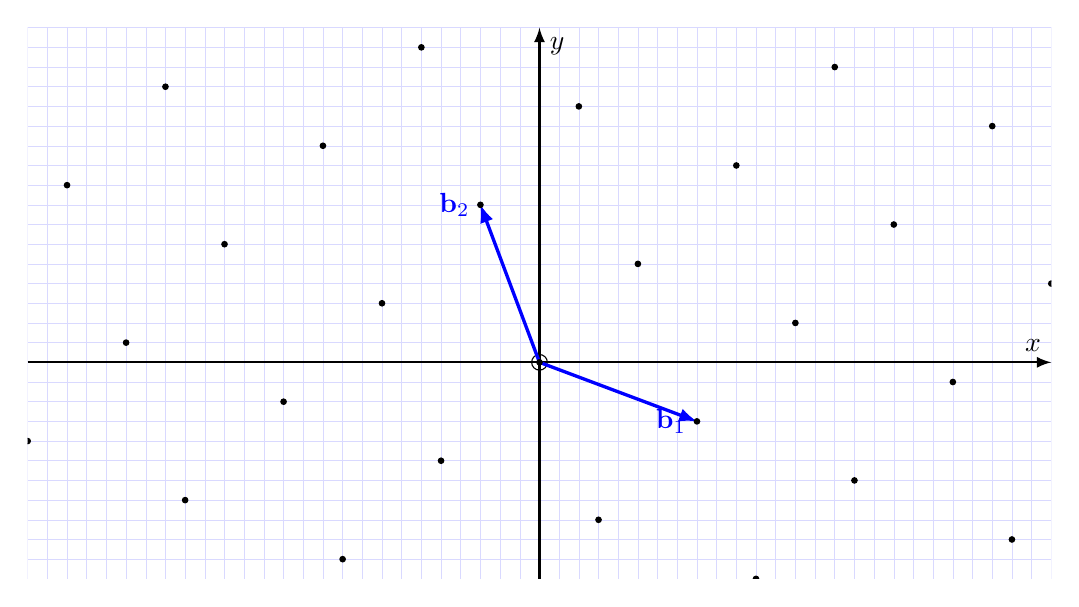
\begin{tikzpicture}[scale=.25]
  \clip(-26,-11)  rectangle (26,17);
   \coordinate (Origin) at (0,0); 
   \coordinate (Bone) at (8,-3);
   \coordinate (Btwo) at (-3,8);
     \draw[style=help lines,color=blue!15] (-26,-20) grid[step=1cm] (26,20);
%     \draw[style=help lines,thin,dotted] (-26,-20) grid[step=1cm] (26,20);
   \draw[thick,-latex] (-26,0) -- (26,0) node [above left] {$x$};
  \draw[thick,-latex] (0,-17) -- (0,17) node [below right] {$y$};
  \node[draw,circle,inner sep=2pt] at (0,0) {};     
  \draw [very thick,-latex,blue] (Origin)    -- (Bone) node [left] {$\vec b_1$};
     \draw [very thick,-latex,blue] (Origin)   -- (Btwo) node [left] {$\vec b_2$};
  \foreach \y in {-5,-4,...,5}{%Two indices running over each 
      \foreach \x in {-5,-4,...,5}{% node on the grid we have drawn
    \node[draw,circle,inner sep=.7pt,fill] at (8*\x-3*\y,-3*\x+8*\y) {};
    }
    }
 \end{tikzpicture}
\end{center}
\end{figure}

Lattices can be defined in several ways, and it is useful to have at least the two following definitions for them. The first definition is explicit: it declares a lattice as the set of {\em integers} linear combinations of a {\em basis} $\vec B$.


\begin{definition}[Lattice, explicit]
If $\vec B = [\vec b_1 \dots \vec b_n ]$ is a matrix with linearly independent column vectors, we call lattice the set \[  \cL(\vec B) = \vec B \cdot \Z^n = \{\vec B \vec z : \vec z \in \Z^n\} \]
\end{definition}

The second definition is implicit, and define a lattice as a discrete subgroup of the Euclidean vector space $\R^m$.

\begin{definition}[Lattice, implicit]
A lattice $L \subset \R^m$ is a discrete subgroup of the Euclidean vector space $\R^m$; that is
$L$ is a non-empty subset of $\R^m$ such that:
\begin{itemize}
\item for any $\vec x,\vec y \in L$, $\vec x - \vec y \in L$ ($L$ is a group)
\item $\vec 0$ is isolated in $L$ that is, there exists a radius $r$ such that $r \cdot \Ball$, 
the centered $\ell_2$ open ball of radius $r$, contains no other lattice point than $\vec 0$: $r \cdot \Ball \cap L = \{ \vec 0 \}$.
\end{itemize}
The dimension $m$ of the vector space containing the lattice is called the embedding dimension of the lattice $L$.
The first minima $\lambda_1(L) > 0 $ of a lattice is the largest radius $r$ as above:
 $\lambda_1(L) = \sup \{r\in \R : r \cdot \Ball \cap L = \{ \vec 0 \}\} = \min_{\vec x \in L\setminus \{\vec 0\}} \norm{\vec x}$.
\end{definition}

While the first definition is simpler, the second definition is also very useful, as it does not require to provide an explicit basis. For example, using the second definition, it is trivial to see that the intersection $L_1 \cap L_2$ is a lattice if both $L_1$ and $L_2$ are lattices. But showing that both definition are equivalent requires a bit of effort \dots

\begin{theorem}[Equivalence of the two definitions]
Both definitions for lattices are equivalent, that is
\begin{itemize}
  \item[a.] If $\vec B \in \R^{m \times n}$ is a matrix with linearly independant column, show that $\cL(\vec B)$ is a discrete subgroup of $\R^m$
  \item[b.] If $L$ is a discrete subgroup of $\R^m$, then there exists a basis $\vec B^{m \times n}$ such that $\cL(\vec B) = L$.
\end{itemize}
\end{theorem}
\begin{problem}
  Prove the above theorem, with the help of the definitions and propositions developed below.
\end{problem}

Lattice are therefore discrete analogues of vector spaces. Both structures share some properties: for example, they both have bases. As vector spaces, lattices can have {\em many different basis}. In fact, for vector-spaces, two basis define the same vector space if and only if there is an invertible matrix sending one to the other. The situation is similar with lattices, but the transition matrices are exactly the unimodular matrices.


\begin{proposition}[Relation between basis]
\label{prop:existence_of_basis}
For any lattice $L \subset \R^m$ of dimension $n$,
if $\vec B$ and $\vec B'$ are both basis of $L$, there exists an integer matrix $\vec U \in \Z^{n \times n}$
such that $\vec B = \vec B' \vec U $ and $\det(\vec U) = \pm 1$.
\end{proposition}
\begin{proof}
Let $\vec B$ and $\vec B'$ be bases of $L$. In particular, any vector $\vec b \in \vec B$ belongs to $L$, therefore, it
can be written as a linear combination of vectors of $\vec B'$: there exists an integer matrix $\vec U \in \Z^{n \times n}$ such 
that $\vec B =  \vec B'\vec U$. Similarly, there exists $\vec U' \in \Z^{n \times n}$ {\em s.t.} $\vec B' = \vec B \vec U'$.
We obtain $\vec B = \vec B \vec U \vec U' $, which implies $\vec U \vec U' = \Id_n$ because $\vec B$ has linearly
independent vectors. We conclude that $\det(\vec U) \cdot \det(\vec U')=1$; which implies $\det(\vec U) = \det(\vec U') = \pm 1$
since $\det(\vec U)$ and $\det(\vec U')$ are integers.
\end{proof}


As for vector spaces, one can define the dimension of a lattice.

\begin{definition}[Dimension of a Lattice]
The dimension of a lattice  $L \subset \R^m$ is the dimension $n\leq m$ of the vector space it spans: $\Span_\R(L)$. Alternatively, if the lattice $L$ admits a basis $\vec B \in \R^{m \times n}$ then the dimension of $L = \cL(\vec B)$ is $n$.

If the dimension $n$ of $L$ equals the embedding dimension $m$, then we say that the lattice $L$ is full-rank.
\end{definition}

Finally, analog to sub-vector spaces also exist:
\begin{definition}[Sub-lattice]
If $L,L' \subset \R^m$ are both lattices, we say that $L'$ is a sublattice of $L$ if $L' \subset L$. 
If $L$ is $n$-dimensional, then $L'$ is $n'$-dimensional for some $n' \leq n$, and $\lambda_1(L') \geq \lambda_1(L)$.
\end{definition}

\section{Fundamental domains and volume}
\label{sec:fundamental_domains}

Given a basis of a lattice, an interesting geometrical object is the fundamental parallelepiped \[\cP(\vec B) = \{ \sum_{i=1}^n w_i \vec b_i : w_i \in \halfinterval\}\] associated with that basis.
The following property can be interpreted geometrically as follows: if $\vec B$ is a basis of a lattice $L$,
then the parallelepiped $\cP(\vec B)$ tiles the space with respect to $L$, that is, the sets $\vec x + \cP(\vec B)$
for $\vec x \in L$ covers the whole vector space $\Span_\R(L)$, and those shifted sets do not overlaps. This is depicted in Figure~\ref{fig:tile}.

\begin{figure}
\caption{Tiling of the space with $\cP(\vec B)$}
\label{fig:tile}
\begin{center}
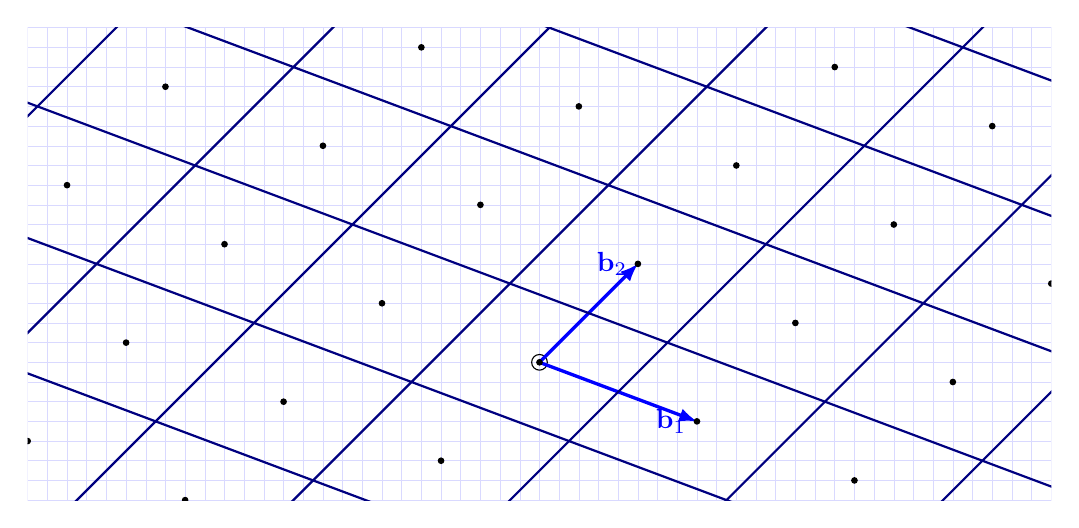
\begin{tikzpicture}[scale=.25]
  \clip(-26,-7)  rectangle (26,17);
   \coordinate (Origin) at (0,0); 
   \coordinate (Bone) at (8,-3);
   \coordinate (Btwo) at (5,5);
   \coordinate (p) at (12,12);
   \coordinate (v) at (10,10);
     \draw[style=help lines,color=blue!15] (-26,-9) grid[step=1cm] (26,23);
%     \draw[style=help lines,thin,dotted] (-9,-9) grid[step=1cm] (23,23);
  \node[draw,circle,inner sep=2pt] at (0,0) {};     
 \draw [very thick,-latex,blue] (Origin)    -- (Bone) node [left] {$\vec b_1$};
 \draw [very thick,-latex,blue] (Origin)   -- (Btwo) node [left] {$\vec b_2$};
  \foreach \y in {-4,-3,...,5}{%Two indices running over each 
      \foreach \x in {-5,-4,...,5}{% node on the grid we have drawn
    \node[draw,circle,inner sep=.7pt,fill] at (8*\x-3*\y,-3*\x+8*\y) {};
    \draw[blue!50!black,thick] (8*\x-3*\y +13/2 + 8,-3*\x+8*\y +2/2 -3)  --
          (8*\x-3*\y +13/2    ,-3*\x+8*\y +2/2   )  --
          (8*\x-3*\y +13/2 + 5,-3*\x+8*\y +2/2 +5);
      }   
    }

 \end{tikzpicture}
\end{center}
\end{figure}



\begin{proposition}
\label{prop:basis_fun_dom}
If $\vec B$ is a basis of a lattice $L= \cL(\vec B) \subset \R^m$, then any $\vec x \in \Span_\R(L)$ can be written
uniquely as $\vec x = \vec v + \vec w$ with $\vec v \in L$ and $\vec w \in \cP(\vec B)$ where $\cP(\vec B)$ denotes the
parallelepiped spanned by $\vec B$: $\cP(\vec B) = \{ \sum_{i=1}^n w_i \vec b_i : w_i \in \halfinterval\}$. We denote 
$\vec x \bmod \vec B$ the unique $\vec w$ as above.
\end{proposition}
\begin{proof}
One can uniquely write $\vec x = \sum x_i \vec b_i$	for $x_i \in \R$ since $\vec B$ is a $\R$-basis
of the vector space $\Span_\R(L)$. For the existence, simply choose $\vec v = \sum \lfloor x_i \rceil \vec b_i$
and $\vec w = \sum (x_i - \lfloor x_i \rceil) \vec b_i$. For uniqueness, decompose $\vec v = \sum v_i \vec b_i$
where $v_i \in \R$ and $\vec w = \sum w_i \vec b_i$ for $w_i \in \halfinterval$. Since the vectors of $\vec B$ are linearly independent,
$\vec x = \vec v + \vec w$ implies $x_i = v_i + w_i$ for all indexes $i$; the only decomposition of $x_i$ as a sum
of an integer and a real in $\halfinterval$ is indeed $v_i = \lfloor x_i \rceil$ and $w_i = x_i - \lfloor x_i \rceil$.
\end{proof}

One note that for two bases $\vec B, \vec B'$ of the same lattice, the volume 
$\Vol(\cP(\vec B)) = \sqrt{\det(\vec B^t \vec B)} $ of $\cP(\vec B)$ is equal to the volume of $\cP(\vec B')$, simply because $\vec B' = \vec B \vec U$ for some matrix $\vec U$ of determinant $\pm 1$:

\[\Vol(\cP(\vec B')) = \sqrt{\det(\vec B'^t \vec B')} = \sqrt{\det(\vec U^t \vec B^t \vec B \vec U)} = \sqrt{\det(\vec U^t) \det(\vec B^t \vec B) \det(\vec U)} = \Vol(\cP(\vec B)). \]


This allows to define the volume of the lattice independently of the choice of the basis:

\begin{definition}[Volume of a lattice]
The volume of a lattice $L$ is defined as $\Vol(L) = \Vol(\cP(\vec B))$ where $\vec B$ is any basis of $L$ ($L = \cL(\vec B)$).
\end{definition}

Proposition~\ref{prop:basis_fun_dom} can be restated using the notion of fundamental domain, saying that if $\vec B$ is a basis of $L$,
then $\cP(\vec B)$ is a fundamental domain of $L$. Informally, a fundamental domain of a lattice $L$, is a set
that tiles whole vector space $\Span_\R(L)$. A more complicated fundamental domains is depicted on Figure~\ref{fig:escher}.

\begin{definition}[Fundamental Domain]
\label{def:fundamental_domain}
For a lattice $L$, a set $\cF \subset \Span_\R(L)$ is called a fundamental domain of $L$ if for all $\vec x \in \Span_\R(L)$ there exist a unique decomposition $\vec x = \vec v + \vec f$ where $\vec v \in L$ and where $\vec f \in \cF$.
Alternatively, $\cF$ is a fundamental domain if the union $\bigcup_{\vec v \in L} \cF + \vec v$ is a disjoint union, and if this union is equal to $\Span_\R(L)$.
% We denote $\vec x \mod \cF$ the unique such $\vec w$.
\end{definition}

\begin{figure} 
 \caption{Fundamental domains in Escher's art work}     
 \label{fig:escher}
\centering
{\includegraphics[width=5cm]{pic/escher2.png}} \quad
{\includegraphics[width=5cm]{pic/escher2_fundamental.png}}
\end{figure}


\section{Gram-Schmidt orthogonalization}

Before going on, please let us introduce two new notations. If $V$ is a sub-vector space of $\R^m$, then $\pi_V : \R^m \rightarrow V$ denotes the orthogonal projection onto $V$. Also, for a matrix $\vec B = [\vec b_1 \dots \vec b_n]$ we will denote $\vec B^{}_{[k]} = [\vec b_1 \dots \vec b_k]$ the partial matrix from column $1$ to $k$.


The Gram-Schmidt orthogonalization (GSO) is an algorithm that transforms any basis $\vec B$
of a vector space to an orthogonal basis $\vec B^\star$ of the same vector space. Yet, if $\vec B$
is a basis of a lattice $L$, $\vec B^\star$ is not necessarily a basis of the same lattice since,
all the $\vec b^\star_i$'s may not belong to $L$ for any index $i>1$; in general, and unlike vector
spaces, lattices do not admit orthogonal base. Yet the Gram-Schmidt of a lattice basis remain a 
useful object. In particular, when it will come to using basis a to find close
vector, the GSO can provide a better solution.

\begin{definition}[Gram-Schmidt Orthogonalization (GSO)]
\label{def:GSO}
Let $\vec B = [\vec b_1 \dots \vec b_n] \in \R^{m \times n}$ be a matrix. The Gram-Schmidt Orthogonalization (GSO)
$\vec B^\star = [\vec b^\star_1 \dots \vec b^\star_n] \in \R^{m \times n}$ is defined as follows:
\begin{align*}
	\vec b^\star_1 & = \vec b^{}_1 \\
	\vec b^\star_i & = \vec b^{}_i - \pi_{\Span_\R(\{\vec b_1 \dots \vec b_{i-1}\})}(\vec b^{}_i) \\ & = \pi_{\{\vec b_1 \dots \vec b_{i-1}\}^{\bot}}
	(\vec b_i)
\end{align*}
Note that this recursive definition implies that for any $k \leq n$, $[\vec b^\star_1 \dots \vec b^\star_k]$
is the GSO of $[\vec b_1 \dots \vec b_k]$, in other words $(\vec B^{}_{[k]})^\star = (\vec B_{}^\star)^{}_{[k]} = \vec B^\star_{[k]} $.
\end{definition}

From this definition, we can deduce an algorithm to compute the Gram-Schmidt orthogonalization.


\begin{algorithm}
\caption{Gram-Schmidt algorithm}
\label{alg:GSO}
\begin{algorithmic}[1]
    \REQUIRE A basis $\vec B = [\vec b_1, \dots, \vec b_n]$ of a full-rank lattice $L \subset \R^m$. \\
    \ENSURE The GSO $\vec B^\star$ of $\vec B$
  \FOR{$i=1$ to $n$ } 
  \STATE $\vec b^\star_i \gets \vec b_i$
  \FOR{$j=1$ to $i-1$ } 
  \STATE $\vec b^\star_i \gets \vec b^\star_i - \frac {\ps{\vec b_i^\star}{\vec b_j^\star}}  {\| \vec b_j^\star \|^2} \cdot \vec b_j^\star$
  \ENDFOR
  \ENDFOR
\STATE return $\vec B^\star = [\vec b_1^\star, \dots , \vec b_n^\star]$
  \end{algorithmic}
\end{algorithm}

We easily see that this algorithm performs $O(n^3)$ operations on real numbers (yet it's bit-complexity may be larger if one requires the result with high precision).


\begin{proposition}[Gram-Schmidt Orthogonalization]
For any $n\times m$ real matrix $\vec B$, there exists a unique decomposition $\vec B =  \vec B^\star \cdot \mu$, 
where $\mu=(\mu_{i,j})$ is an $n\times n$ upper-triangular matrix with unit diagonal, $\vec B^\star$ is an $n\times m$ matrix with orthogonal column vectors.
The transition matrix $\mu$ satisfies
\[\mu_{j,i}= \langle \vec b_i\, , \vec b^\star_j \rangle / \Vert \vec b^\star_j \Vert^2 \].
\end{proposition}

In particular, this gives a relation between the GSO of a basis and the volume of a lattice its spans, namely

\begin{corollary}
If $\vec B$ is the basis of a $n$-dimensional lattice $L \subset \R^m$, and $\vec B^\star$ is its GSO,
then \[\Vol(L) = \prod_{i = 1}^n \norm{\vec b^\star_i}\].
\end{corollary}
\begin{proof}
  Simply note that $\Vol(L) = \Vol(\cP(\vec B))$ where
  \[\Vol(\cP(\vec B))^2 = \det((\vec B^\star \mu)^t (\vec B^\star \mu) ) = \det(\mu^t) \det( (\vec B^\star)^t \vec B^\star) \det(\mu) = \Vol(\cP(\vec B^\star))^2 \]
  and that $ \Vol(\cP(\vec B^\star)) = \prod_{i = 1}^n \norm{\vec b^\star_i}$ because the $\vec b^\star_i$'s are orthogonal.
\end{proof}



An interesting property of the GSO $\vec B^\star$, is that, even if it {\em is not a basis} of the 
lattice $\cL(\vec B)$, the parallelepiped it spans is still a fundamental domain of $\cL(\vec B)$, as shown in figure~\ref{fig:tilegso}.

\begin{figure}
\caption{Tiling of the space with $\cP(\vec B^\star)$}
\label{fig:tilegso}
\begin{center}
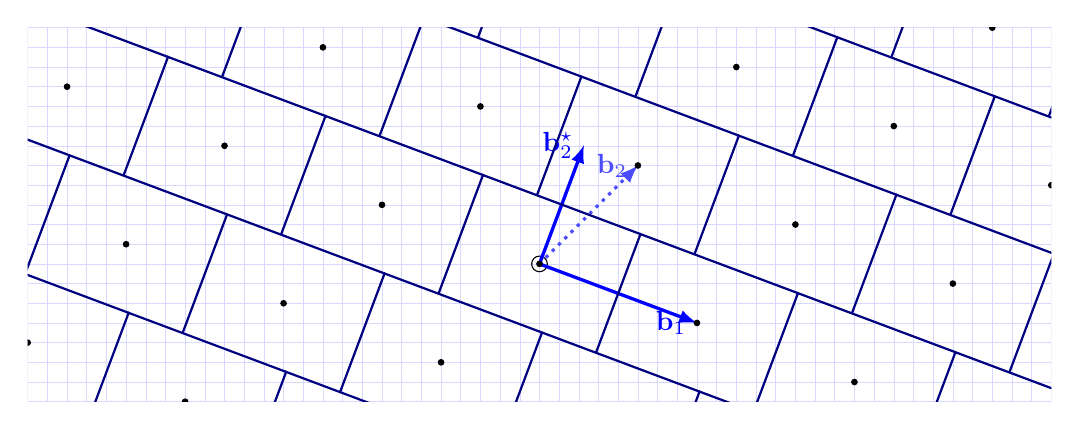
\begin{tikzpicture}[scale=.25]
  \clip(-26,-7)  rectangle (26,12);
   \coordinate (Origin) at (0,0); 
   \coordinate (Bone) at (8,-3);
   \coordinate (Btwo) at (5,5);
   \coordinate (Btwos) at (165/73,440/73);
   \coordinate (p) at (12,12);
   \coordinate (v) at (10,10);
     \draw[style=help lines,color=blue!15] (-26,-9) grid[step=1cm] (26,23);
%     \draw[style=help lines,thin,dotted] (-9,-9) grid[step=1cm] (23,23);
  \node[draw,circle,inner sep=2pt] at (0,0) {};     
 \draw [very thick,-latex,blue] (Origin)    -- (Bone) node [left] {$\vec b_1$};
 \draw [very thick,-latex,blue!70!white, dotted] (Origin)   -- (Btwo) node [left] {$\vec b_2$};
 \draw [very thick,-latex,blue] (Origin)   -- (Btwos) node [left] {$\vec b^\star_2$};
  \foreach \y in {-4,-3,...,5}{%Two indices running over each 
      \foreach \x in {-5,-4,...,5}{% node on the grid we have drawn
    \node[draw,circle,inner sep=.7pt,fill] at (8*\x-3*\y,-3*\x+8*\y) {};
    \draw[blue!50!black,thick] 
          (8*\x-3*\y - 165/146 - 8/2,-3*\x+8*\y - 440/146 + 3/2)  --
          (8*\x-3*\y + 165/146 - 8/2,-3*\x+8*\y + 440/146 + 3/2)  --
          (8*\x-3*\y + 165/146 + 8/2,-3*\x+8*\y + 440/146 - 3/2);

      }   
    }

 \end{tikzpicture}
\end{center}
\end{figure}



\begin{proposition}
\label{prop:GSObasis_fun_dom}
If $\vec B$ is a basis of an $n$-dimensional lattice $L=\cL(\vec B) \subset \R^m$ and if $\vec B^\star = \vec B \mu^{-1}$ is the GSO of $\vec B$,
then $\cP(\vec B^\star)$ is a fundamental domain.
\end{proposition}
The proof is interesting because we can deduce an algorithm from it, called the nearest plane algorithm, that we will see later.

\begin{proof}
We proceed by induction. Recall from the definition of GSO that $(\vec B_{[k]})^\star = (\vec B^\star)_{[k]}$.
For a one dimensional lattice $\vec B = [\vec b]$, we have $\vec B^\star = \vec B$, so 
$\cP(\vec B^\star)=\cP(\vec B)$ is a fundamental domain of $\cL(\vec B)$.

Now, consider an $n$-dimensional lattice $\cL(\vec B)$. By induction, $\cP(\vec B_{[n-1]}^\star)$ is a fundamental domain
of $\cL(\vec B_{[n-1]})$. Let $\vec x$ be an arbitrary vector in  $\Span_\R(L)$, it can be written as 
$\vec x' + x_n \vec b^\star_n$ where $\vec x \in \Span_\R(\vec B_{[n-1]})$ and $x_n \in \R$. 
Set $x'_n = \lfloor x_n \rceil \in \Z$, and rewrite 
\[\vec x = \underbrace{\vec x' + (x_n -x'_n) (\vec b_n - \vec b_n^\star)}_{\vec v\; \in\;  \Span_\R(\vec B_{[k-1]})} + \underbrace{x'_n \vec b_n}_{\in \cL(\vec b_n)} + \underbrace{(x_n -x'_n) \vec b^\star_n}_{\in \cP(\vec b_n^\star)}.\]

Note that $\vec v = \vec x' + (x_n -x'_n) (\vec b_n - \vec b_n^\star)$ belongs to $\Span_\R(\vec B_{[k-1]})$,
therefore, by induction it can be written as $\vec v = \vec y + \vec z$ where $\vec y \in \cL(\vec B)$ and
$\vec z \in \cP(\vec B^\star_{[n-1]})$. We conclude on existence by checking that 
$\vec x = (\vec v + x'_n \vec b_n) + (\vec z + (x_n -x'_n) \vec b^\star_n)$, and that
$ (\vec v + x'_n \vec b_n) \in \cL(\vec B)$ and $(\vec z + (x_n -x'_n) \vec b^\star_n) \in \cP(\vec B^\star)$.

For uniqueness, consider two decompositions of $\vec x = \vec B\vec y + \vec B^\star \vec z = \vec B \vec y' + \vec B^\star \vec z'$ where $\vec y, \vec y' \in \Z^n$ and $\vec z, \vec z \in \halfinterval^n$. To prove uniqueness, we should show that $\vec y = \vec y'$ and $\vec z = \vec z'$. Consider the quantity $\ps{\vec x}{\vec b^\star_n}$, 
because $\vec b_n^\star$ is orthogonal to all $\vec b_i^\star$ and $\vec b_i^\star$, we have:
\[ \ps{\vec x}{\vec b^\star_n} = y_n \ps{\vec b_n}{\vec b_n^\star} + z_n \ps{\vec b_n^\star}{\vec b_n^\star}
= y'_n \ps{\vec b_n}{\vec b_n^\star} + z'_n \ps{\vec b_n^\star}{\vec b_n^\star}. \] It remains to note
that $\ps{\vec b_n}{\vec b_n^\star} = \ps{\vec b_n^\star}{\vec b_n^\star} = \norm{\vec b_n^\star}^2$,
to deduce $y_n = y'_n$ and $z_n = z'_n$. To conclude, it remains to apply the induction hypothesis on
$\vec x - (y_n \vec b_n + z_n \vec b^\star_n)$ which belongs to $\cL(\vec B_{[n-1]})$.
\end{proof}

\section{Finding close vectors}

An interesting algorithmic problem related to a lattice is the close vector problem: given a basis of a lattice $L \subset \R^m$, and a target point $\vec t \in \R^m$, find a vector $\vec v \in L$ such that $\vec v$ is close to $\vec t$.

This problem has many variant, for example the hardest variant is the closest vector problem, and this variant is known to be NP-hard, and it relates to a geometrical object called the ``Voronoi cell''. 

The variants that we will use for cryptography are described below. Those variants are not known to be NP-hard, but are still quite hard to solve, and typically require exponential time to solve (unless one is equipped with a {\em good basis} of $L$, as we shall see below).

This first version asks one to find a solution at distance at most $d$, and it is implicitly assumed that $d$ is large enough so that at least one solution exists for any target vector $\vec t$. For a more formal understanding of this implicit condition, please refer to the notion of {\em covering radius} of a lattice, as defined in Lecture X of~XXX. One note that the larger $\eta$ is, the easier the problem gets, and gets trivial for $\eta = \infty$.

\begin{definition}[Close vector problem: $\delta$-CVP]
  Given the basis $\vec B \in \R^{n \times n}$ of a (full-rank) lattice $L \in \R^n$, and a target $\vec t \in \R^n$ find $\vec v \in L$ such $\|\vec t - \vec v\| \leq \delta$.
\end{definition}



A second version of this problem useful for cryptography, especially encryption is the Bounded-Distance Decoding problem (BDD). In this version, one is asked to find a very close lattice point, at distance at most $d \leq \lambda_1(L)/2$. Such condition ensures that at {\em most one solution} exists, and for most targets $\vec t \in \R^m$ there will be no such solutions. The BDD problem is therefore a problem with a promise that $\vec t$ is unusually close to the lattice $L$. This version is better understood as a decoding task, that is, given a noised version $\vec v + \vec e$ ($\vec e$ is a small error) of a vector $\vec v \in L$ one must remove the noise $\vec e$ to recover the ``message'' $\vec v$. This problem is somehow a dual problem to $\delta$-CVP. In particular, this problem become easier when $\delta$ decreases, and gets trivial when $\delta = 0$. 

\begin{definition}[Bounded Distance Decoding Problem: $\eta$-BDD]
  Given the basis $\vec B \in \R^{n \times n}$ of a (full-rank) lattice $L \in \R^n$, and a target $\vec t = \vec v + \vec e$ for some $\vec v \in L$ and some small $\vec e \in \R^n$, $\|\vec e\| \leq \eta < \lambda_1(L)/2$, recover $\vec v$ (or equivalently $\vec e$).
\end{definition}

As mentioned before, those problems can be solved with basis of sufficient quality. For example there is a very simple algorithm (called the round'off algorithm) that, given a target $\vec t$ finds a solution $\vec v$ such that $\vec t -\vec v \in \cP(\vec B)$. We say that this algorithm is associated with the fundamental domain $\cP(\vec B)$.


\begin{algorithm}
\caption{Round'off algorithm}
\label{alg:RoundOff}
\begin{algorithmic}[1]
    \REQUIRE A basis $\vec B$ of a full-rank lattice $L \subset \R^n$, a target point $\vec t \in \R^n$. \\
    \ENSURE A decomposition $\vec t = \vec v + \vec f$ where $\vec v \in L$ and $\vec w \in \cP(\vec B)$
  \STATE $\vec x \gets \vec B^{-1} \vec t$ 
  \STATE $\vec y \gets (\lfloor x_1 \rceil, \dots , \lfloor x_n \rceil)$ 
  \STATE $\vec v \gets \vec B \vec y$
  \STATE $\vec f = \vec t - \vec v$
\STATE return $(\vec v, \vec f)$
  \end{algorithmic}
\end{algorithm}

What is the ``quality of the output'', i.e. how large is $\vec f = \vec t - \vec v$ is ? Well, we know that $\vec f \in \cP(\vec B)$, that is $\vec f = \sum \vec b_i r_i$ for some $r_i \in \halfinterval$. By the triangle inequality we deduce
\[\|\vec f\| \leq \frac 1 2 \sum \|\vec b_i\|.\]

  We see that the quality of the output highly depends on the ``quality of the basis''. The conclusion is that if we have a good basis, that is a basis such that $2 \sum \|\vec b_i\| \leq \delta$, then we can solve $\delta$-CVP quite efficiently: the above algorithm only requires $O(n^2)$ operations. But finding a good basis is also a hard problem: one must have a very special knowledge about the lattice $L$ to solve those $\delta$-CVP problems.


The above algorithm was rather simple, and has rather poor quality. It is possible to improve the quality a bit by using the Gram-Schmidt orthogonalization. This time we will obtain a solution $\vec v$ such that $\vec t -\vec v \in \cP(\vec B^\star)$: this new algorithm (the nearest plane algorithm) is associated with the fundamental domain $\cP(\vec B^\star)$. As mentionned earlier, this algorithm can be viewed as an algorithmic version of (the existence part of) the proof of Proposition~\ref{prop:GSObasis_fun_dom}, saying that $\cP(\vec B^\star)$ is indeed a fundamental domain.

\begin{algorithm}
\caption{Nearest Plane Algorithm}
\label{alg:BabaiNearestPlane}
\begin{algorithmic}[1]
    \REQUIRE A basis $\vec B$ of a full-rank lattice $L \subset \R^n$, its GSO $\vec B^\star$, and a target point $\vec t \in \R^n$. \\
    \ENSURE A decomposition $\vec t = (\vec v + \vec f)$ where $\vec v \in L$ and $\vec w \in \cP(\vec B^\star)$
    \STATE $\vec f \gets \vec t$
    \STATE $\vec v \gets \vec 0$
  \FOR{$i=n$ downto $1$ } 
    \STATE $y \gets \ps{\vec t}{\vec b^\star_i} / \|\vec b^\star_i\|^2$
    \STATE $z_i = \lfloor y \rceil$
    \STATE $\vec f \gets \vec f - z_i \vec b_i$
    \STATE $\vec v \gets \vec v + z_i \vec b_i$
  \ENDFOR
\STATE return $(\vec v,\vec f)$
  \end{algorithmic}
\end{algorithm}

This algorithm also runs in time $O(n^2)$ but can solve $\delta$-CVP for a potentially smaller $\delta$. Another advantage is that it is also easier to find a sufficient condition for this algorithm to solve $\eta$-BDD.

\begin{proposition}
\label{prop:npa}
  The Nearest Plane Algorithm with basis $\vec B$ solves:
  \begin{itemize}
    \item $\delta$-CVP for any $\delta \geq \frac 1 2 \sqrt {\sum \| \vec b_i^\star \|^2}$
    \item $\eta$-BDD for any $\eta \leq \frac 1 2 \min \| \vec b^\star_i \|$.
  \end{itemize}
\end{proposition}
\begin{proof}
The details are left as an exercise. For the first statement, one should use the Pythagorean identity, exploiting the orthogonality of the basis $\vec B^\star$. For the second identity, on should prove that the ball of radius $d$ is included in $\cP(\vec B^\star)$.
\end{proof}

\section{Good bases, bad bases, and cryptography}

As we have seen above, the ability to solve the $\delta$-CVP and $\eta$-BDD problems highly depends on the quality of the basis that one is given. And it is also a hard problem, given bad basis of a lattice to construct a good one. But one thing that can be done, is to directly construct a lattice $L$ as the lattice $\cL(\vec G)$ for some good basis $\vec G$ that one chooses !

This very idea gives a foundation to build asymmetric cryptography from lattices. It goes as follows:
\begin{itemize}
  \item Alice chooses a good basis $\vec G$, and set $L = \cL(\vec G)$. She keeps $\vec G$ as a {\em secret key} $sk = \vec G$.
  \item She also derives $\vec B$ a bad basis of the same lattice: $\cL(\vec B) = \cL(\vec G)$.\footnote{ This can be done for example by sampling a random unimodular matrix $\vec U$ and setting $\vec B = \vec G \vec U$. There are better ways to do that, see the Hermite normal form in the lecture X from XXX} She makes $pk = \vec B$ public as her {\em public key}.
  \item Bob uses $\vec B$ to encrypt messages
  \item Alice uses $\vec G$ to decrypt messages.
\end{itemize}



\begin{figure}
\caption{BDD radius using $\vec G$ versus $\vec B$}
\label{fig:decoding}
\center
\begin{tabular}{cc}

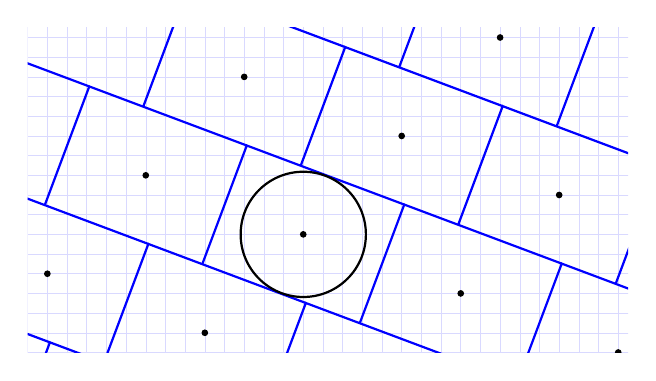
\begin{tikzpicture}[scale=.25]
  \clip(-4,4)  rectangle (26.5,20.5);
   \coordinate (Origin) at (0,0); 
   \coordinate (Bone) at (8,-3);
   \coordinate (Btwo) at (5,5);
   \coordinate (p) at (12,12);
   \coordinate (v) at (10,10);
     \draw[style=help lines,color=blue!15] (-6,4) grid[step=1cm] (27,21);
%     \draw[style=help lines,thin,dotted] (-9,-9) grid[step=1cm] (23,23);
  \node[draw,circle,inner sep=2pt] at (0,0) {};     
% \draw [very thick,-latex,blue] (Origin)    -- (Bone) node [left] {$\vec b_1$};
%     \draw [very thick,-latex,blue] (Origin)   -- (Btwo) node [left] {$\vec b_2$};
  \foreach \y in {-3,-2,...,5}{%Two indices running over each 
      \foreach \x in {-3,-2,...,5}{% node on the grid we have drawn
    \node[draw,circle,inner sep=.7pt,fill] at (8*\x-3*\y,-3*\x+8*\y) {};
    \draw[blue,thick] 
          (8*\x-3*\y - 165/146 - 8/2,-3*\x+8*\y - 440/146 + 3/2)  --
          (8*\x-3*\y + 165/146 - 8/2,-3*\x+8*\y + 440/146 + 3/2)  --
          (8*\x-3*\y + 165/146 + 8/2,-3*\x+8*\y + 440/146 - 3/2);

    
    }
}
\node[draw, thick, circle,inner sep=16pt] at (10,10) {};
 \end{tikzpicture}
&
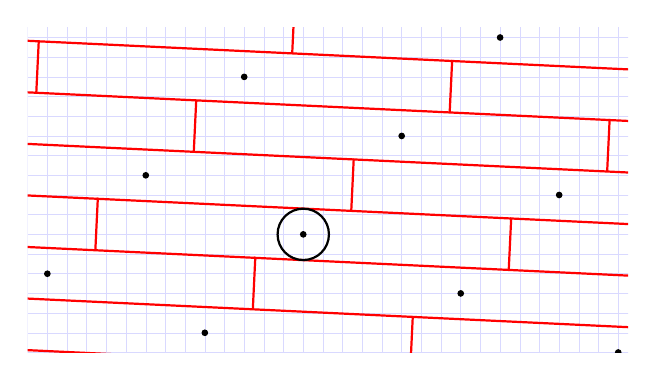
\begin{tikzpicture}[scale=.25]
  \clip(-4,4)  rectangle (26.5,20.5);
   \coordinate (Origin) at (0,0); 
   \coordinate (Bone) at (21,-1);
   \coordinate (Btwo) at (13,2);
   \coordinate (Btwos) at (55/442,1155/442);
   \coordinate (p) at (12,12);
   \coordinate (v) at (23,12);
     \draw[style=help lines,color=blue!15] (-6,4) grid[step=1cm] (27,21);
 %    \draw[style=help lines,thin,dotted] (-9,-9) grid[step=1cm] (23,23);
  \node[draw,circle,inner sep=2pt] at (0,0) {};     
% \draw [very thick,-latex,red] (Origin)    -- (Bone) node [below] {$\vec b_1$};
%     \draw [very thick,-latex,red] (Origin)   -- (Btwo) node [above] {$\vec b_2$};
  \foreach \y in {-3,-2,...,5}{%Two indices running over each 
      \foreach \x in {-3,-2,...,6}{% node on the grid we have drawn
    \node[draw,circle,inner sep=.7pt,fill] at (8*\x-3*\y,-3*\x+8*\y) {};
    \draw[red,thick]  
          (8*\x-3*\y - 55/884 - 21/2,-3*\x+8*\y - 1155/884 + 1/2)  --
          (8*\x-3*\y + 55/884 - 21/2,-3*\x+8*\y + 1155/884 + 1/2)  --
          (8*\x-3*\y + 55/884 + 21/2,-3*\x+8*\y + 1155/884 - 1/2);
    }
    }
    \node[draw, thick, circle,inner sep=2900/442pt] at (10,10) {};
 \end{tikzpicture} \\
  Decoding radius with $\vec G^\star$ & Decoding radius with $\vec B^\star$
\end{tabular}


\end{figure}

But how are messages encrypted and decrypted ? Well, we need to have a gap between the quality of $\vec B$ and $\vec G$. Let $\eta$ be a positive real number such that:
\[ \eta_{\vec B} = \frac 1 2 \min \| \vec b^\star_i \| \ll \eta \leq \frac 1 2 \min \| \vec g^\star_i \| = \eta_{\vec G} . \]

The symbol $\ll$ means ``much smaller than'', and it won't be made formal in this lecture. The reason we need a significant margin is that the nearest plane Algorithm behave better in the average case than in the worst case: the sufficient condition of Proposition~\ref{prop:npa} are not exactly necessary in the average case.

With those conditions, Alice will be able to solve $\eta$-BDD while this will be very hard for anyone else knowing only $\vec B$. This suggest to make the ciphertext an $\eta$-BDD instance, so that only alice can solve it !

More precisely, one would define the encryption function on a message $\vec m \in \{0,1\}^n$ (the message is viewed as a vector of bits) and with the public key $pk = \vec B$ to obtain a ciphertext $\vec c$ as follows:
\[ \vec c = \mathcal E(\vec B, \vec m) = \vec B \cdot \vec m + \vec e\]
where $\vec e$ is a random vector of length $\eta$: $\|\vec e\| = \eta$.

The decryption function will use the Nearest Plane algorithm to remove the error $\vec e$. Alice will use both the good and the bad basis to recover the message.

\[ \vec m' = \mathcal D(\vec G, \vec B, \vec c) = \vec B^{-1} \vec v \quad \text{ where } (\vec v, \vec e') = \text{NearestPlane}(\vec G, \vec G^\star, \vec c). \]

Using Proposition~\ref{prop:npa}, one deduce that $\vec m' = \vec m$: Alice has properly decrypted the ciphertext $\vec c$ to the message right message $\vec m$.

\paragraph{Is the above scheme truly secure ?} We have informally argued that, without the secret key $sk = \vec G$, it should be hard to recover the message $\vec m$. This is unfortunately not so simple, and it is possible to attack this scheme. To see this, one need to start studying what it means precisely for a scheme to be secure in a formal sense, which is left as an exercise for the curious reader.

\begin{problem}
  Learn about the notion of Indistinguishability under Chosen-Plaintext Attacks (IND-CPA security), and show that the above scheme is not IND-CPA secure.
\end{problem}

\section{Provably secure encryption from lattices and beyond}

This lecture meant to give the basic tools to understand lattices, associated algorithms, and the ideas behind lattice based cryptography. Those ideas dates back from the early schemes of Goldreich-Goldwasser-and Halevi and the NTRU schemes (form the late 90').

Since then, the theory of lattice based cryptography has made tremendous progress, in particular by formalizing more precise problems called the Short-Integer-Solution problem (SIS) and the Learning-with-Error problem (LWE). Those problems are intrinsically lattice problems, but are typically presented without speaking of lattices at all ! While this is convenient to build better cryptosystems, this hides a little bit the intuition behind the design of those schemes.

Therefore, we shall finish this lecture with the translation of the LWE problem to a BDD problem. 

\begin{definition}[The Learning with Errors Problem]
  The Learning with Errors Problem, $\text{LWE}_{n,m,q,\chi}$, with $n$ unknown, $m\geq n$ samples, modulo $q$ and with errors distribution $\chi$ is as follows: 
  \begin{itemize}
    \item for a random secret $\vec s$ uniformly chosen in $\Z_q^n$, 
    \item given $m$ samples of the form $(\vec a,b = \ps{\vec s}{\vec a} + e \bmod q)$ where $e \leftarrow \chi$ and $\vec a$ is uniform in $\Z_q^n$, 
    \item recover the secret vector $\vec s$.
  \end{itemize}
\end{definition}

To state this problem in term of lattice, consider the matrix $\vec A = [\vec a_1 \dots \vec a_m]^t$ whose rows are the samples $\vec a_i$, the vector $\vec b = \vec A \vec s  + \vec e$ where $\vec e \leftarrow \chi^m$, and define the LWE lattice.

\begin{definition}[The LWE-lattice]
  For integers parameters $n,m>n ,q$, and for a $\text{LWE}_{n,m,q,\cdot}$ instance matrix $\vec A \in \Z_q^{m \times n}$, the LWE-lattice associated to the instance $(\vec A,\vec b)$, $\cL^{q}(\vec A^t)$, is defined as:
  \[ \cL^{q}(\vec A) = \left\{ \vec v \in \Z^m : \exists \vec s \in \Z_q^n \text{s.t.} \, \vec v \equiv \vec A \vec s \bmod q\right\} .\]
  In other words, $\cL^{q}(\vec A)$ is the lattice generated by the column vectors of $\vec A$ and the column vectors of $q \Id_m$, {\em i.e.} the canonical vectors scaled by $q$.
\end{definition}

When $\vec e$ is small, the problem can now be seen as follows: given a point $\vec b$ close to a random lattice point $ \vec A \vec s \bmod q$, one is asked to recover $\vec s$. The problem LWE is a variant of BDD for a certain distribution of lattice and errors. We will conclude with the following exercise:
\begin{problem}
  Prove that for any matrix $\vec A \in \Z_q^{m \times n}$, $\cL^{q}(\vec A)$ is a lattice, that it has dimension $m$ and volume $q^{m-n}$. 
\end{problem}
\paragraph{Hint:} For the volume, first prove that if $L'$ is a sublattice $L$, then the quotient group $L/L'$ has size $\Vol(L')/\Vol(L)$.
\end{document}